\documentclass{article}
% \usepackage{hyperref}

\usepackage{titlesec}
\usepackage{titling}
\usepackage{multicol}
% \usepackage{hyperref}
\usepackage[margin=0.3in]{geometry}

\usepackage{MnSymbol}
\usepackage{amsmath} 
\usepackage{graphicx} 
\usepackage{eso-pic}
\usepackage[hidelinks]{hyperref}

\usepackage{ifthen}
\newboolean{showProjectlinks}
\setboolean{showProjectlinks}{true}

\titleformat{\section}
{\large\uppercase}
{}
{0em}
{}[\titlerule]

\titleformat{\subsection}[runin]
{\bfseries}
{}
{1em}
{}[]

\renewcommand{\maketitle}{
    \begin{flushleft}        
        {\huge\rmfamily
        \theauthor}\newline
        \vspace{0.1em}
        \textit{teetangh@gmail.com -- github.com/teetangh}\newline
        \textit{Contact No. -- +91-8800441954}\newline
        \textit{Manipal Institute of Technology}\newline
        \textit{B.Tech in \textbf{Computer Science \& Engineering}}
        \textit{2018 - 2022}\newline
        \textit{Minor in \textbf{Computational Intelligence}}\newline
        \textit{CGPA: 8.45/10}\newline
    \end{flushleft}

}


\titlespacing*{\subsection}
{0em}
{0em}
{0em}


%%%%%%%%%%%%%%%%%%%%%%%%%%%%%%%%%%%%%%   DOCUMENT  %%%%%%%%%%%%%%%%%%%%%%%%%%%%%%%%%%%%%%%%%%%%%%%%%%%%%%%


\begin{document}
\thispagestyle{empty}  % for no page numbering

% \begin{multicols}{2}
%     \title{Resume}
%     \author{Kaustav Ghosh}
%     \maketitle
%     \begin{flushright}
%         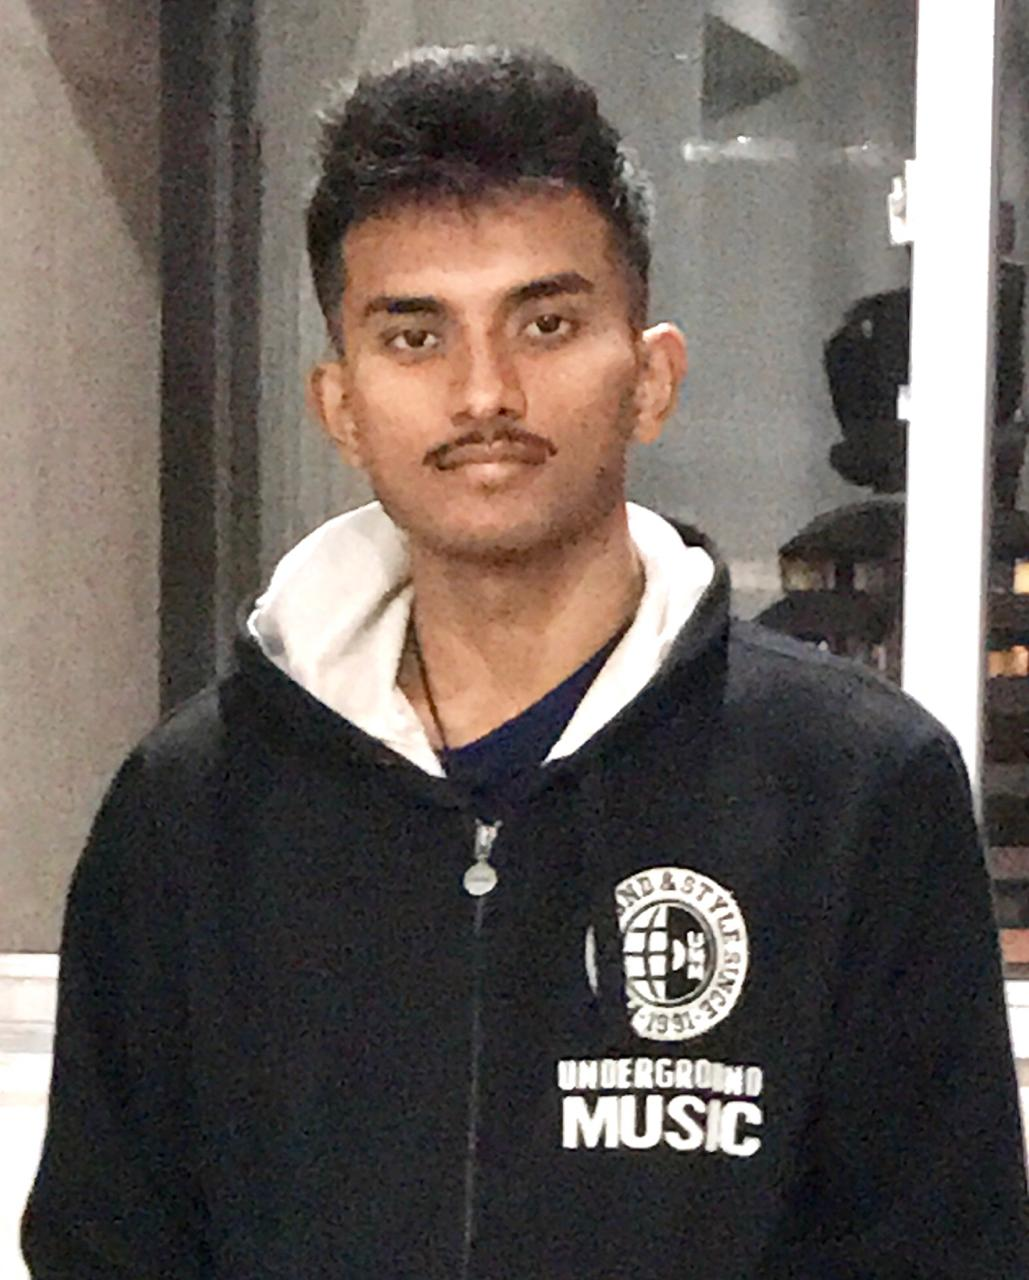
\includegraphics[height=3cm]{kaustav2.jpeg}
%     \end{flushright}
% \end{multicols}

\begin{center}
    \huge{Kaustav Ghosh}

    \normalsize{
        \textit{
            \href{https://www.github.com/teetangh}{GitHub} \(|\)
            \href{https://www.linkedin.com/in/kaustav-ghosh-1538651bb/}{LinkedIn} \(|\)
            teetangh@gmail.com \(|\)
            Gugraon,India \(|\)
            +91-8800441954
        }}
\end{center}

\section*{Education}
% \subsection*{
%     Manipal Institute of Technology
%     \begin{flushright}
%         \text{2018-2022}
%     \end{flushright}
%     }

% Left \hfill Center \hfill Right
\textbf{Manipal Institute of Technology} \hfill \textit{2018-2022}
\textmd{\newline \textit{BTech in Computer Science and Engineering specializing in Computational Intelligence}} \hfill \textit{CGPA: 8.45/10}
\textmd{\newline \textit{Interests: Artificial Intelligence and Robotics}}

\section*{Internships}

\begin{itemize}
    \item{\textbf{\large{Samsung R\&D, Bangalore - Software Engineer Intern, IoT Products \& Analytics}}} \hfill \textit{Jun'21-Jul'21}
          \newline
          \textit{- Developed and implemented MQTT bridge functionality in Moquette, an open-source lightweight Java MQTT broker}
\end{itemize}


\begin{itemize}
    \item{\textbf{\large{Microsoft Student Partners-Machine Learning Intern}}} \hfill \textit{Apr'20-Jun'20}
          \newline
          \textit{-Guided a team of 10 individuals to collaborate and accomplish a Regression task of price prediction of used cars in a machine learning pipeline through Exploratory Data Analysis,Feature Engineering and Model Building.}
          \ifthenelse{\boolean{showProjectlinks}}{
              \textbf{Projects:}\href{https://github.com/teetangh/Microsoft-Machine-Learning-Internship/blob/master/MINOR\%20PROJECT/Microsoft_Minor_Project_v2.ipynb}{\text{[Minor]}}.
              \href{https://github.com/Microsoft-ML-Internship-Team/Major-Project-Submissions}{\text{[Major]}}.
          }{}

\end{itemize}


\begin{itemize}
    \item{\textbf{\large{Qbotics Labs - ROS Engineer Intern}}}\hfill \textit{Jul'20-Aug'20}
          \newline
          \textit{- Constructed a Differential Drive with caster wheel from scratch using URDF and XACRO files and mounted the same with laser scanner , IMU and Velodyne Puck VLP-16 Lidar and simulated the same in Gazebo and Webots}
          \ifthenelse{\boolean{showProjectlinks}}{\textbf{Project:}
              \href{https://github.com/teetangh/Qbotics-Labs-Internship-Differential-Drives}{\text{[Repository]}}.
          }{}

\end{itemize}
% \begin{itemize}
%     \item{\textbf{\large{United Nations TakenMind - Data Analytics Intern}}}
%           \newline
%           \textit{- Performed Exploratory Data Analysis techniques using Matplotlib and
%               Implemented several boxplots,countplots,heatmaps on several data-sets using Seaborn }
% \end{itemize}


% \begin{itemize}
%     \item{\textbf{\large{Ineuron Deep Learning with Masters in Computer Vision and Natural Language Processing}}}
%           \newline
%           \textit{- Postponed due to Covid Situation }
% \end{itemize}

\section*{Research Projects}
\begin{itemize}
    \item{\textbf{\large{Samsung PRISM - Intelligent Ranking for Dynamic Restoration in Next Generation Wireless Networks}}} \hfill \textit{Sep'20-Mar'21}
          \newline
          \textit{- Implemented Machine Learning algorithms and Feature Engineering techniques to predict KPI values for eNodeB-s and consequently a ranking system
              to orderly restore them during network failure.}
\end{itemize}

\section*{Academic Projects}
\begin{itemize}
    \item{\textbf{\large{Compiler Frontend for subset of C-Language}}}
          % Don't know why indentation is not working
          \newline
          \textit{- Coded a \textbf{Lexical Analyser} that extracts tokens from a C source file and a \textbf{Symbol Table Generator} to store information of identifiers and functions and a \textbf{Recursive Decent Parser} that semantically parses the grammar for subset of C-Language by analysing the tokens generated by a Lexical Analyser}
          \ifthenelse{\boolean{showProjectlinks}}{\textbf{Code:}
              \href{https://github.com/teetangh/Kaustav-CSE-LABS-and-Projects/blob/main/Sem05-Compiler-Design-LAB/LAB\%2004/lab04_symbol_table_lexical_analyser_complete.c}{\text{[Lexical Analyser + Symbol Table]}}.
              \href{https://github.com/teetangh/Kaustav-CSE-LABS-and-Projects/blob/main/Sem05-Compiler-Design-LAB/LAB\%200789/lab09_RDP_main.c}{\text{[Recursive Decent Parser]}}.
          }{}
    \item{\textbf{\large{Mini Games based on Backtracking}}}
          \newline
          \textit{- Coded a \textbf{Crossword Solver} that takes a 10*10 grid and word list and outputs a grid with the words accurately filled}
          \newline
          \textit{- Coded a \textbf{Sudoku Solver} that takes a partially filled 9*9 Sudoku grid and outputs a solution so that every row, column and nine 3x3 sub-grids contains exactly 1 instance of the digits from 1 to 9.}
          \ifthenelse{\boolean{showProjectlinks}}{\textbf{Code:}\href{https://github.com/teetangh/competitive-programming/blob/main/CodeZen/03\%20Algorithms\%20and\%20Competitive\%20Programming/11\%20Backtracking/prog004crosswordSolver.cpp}{\text{[Crossword Solver]}}.\href{https://github.com/teetangh/competitive-programming/blob/main/CodeChef/Public/Code\%20Marathon/sudokuSolver.cpp}{\text{[Sudoku Solver]}}.
          }{}
    \item{\textbf{\large{Machine Learning Algorithm Implementations}}}
          \newline
          \textit{- Implemented basic machine learning algorithms such as Linear Regression, K-Nearest Neighbours, Logistic Regression,K-Means Clustering from scratch without existing machine learning libraries. % Currently implementing gradient descent algorthims
          }\ifthenelse{\boolean{showProjectlinks}}{\textbf{Code:}
              \href{https://github.com/teetangh/Kaustav-AI-workspace/tree/main/ML}{\text{[AI-workspace]}}.
          }{}
    \item{\textbf{\large{Time Series Forecasting, Data Analysis and Web Scraping on Covid-19 data}}}
          % Don't know why indentation is not working
          \newline
          \textit{- Prepared a complete Data Analysis report on the World-wide COVID-19 attack statistics and used the Facebook's fbprophet Time-series Forecasting library to speculate the number of active corona victim cases in the upcoming days.}
          \ifthenelse{\boolean{showProjectlinks}}{\textbf{Code:}
              \href{https://github.com/teetangh/FinlandLabs-IITR-COVID-19-Analysis}{\text{[Project]}}.
          }{}
    \item{\textbf{\large{Food Labs Robotics Startup Competition}}}
          \newline
          \textit{- Designed, modelled, constructed and
              Assembled a plethora of sensors and Robots across multiple software platforms like
              freeCad,Blender,Gazebo and also fabricated a Defense Building from scratch using Gazebo World Editor}
          \ifthenelse{\boolean{showProjectlinks}}{\textbf{Repository:}
              \href{https://github.com/teetangh/FoodLabs-ROS-Startup-Competition}{\text{[Project]}}.
          }{}
    \item{\textbf{\large{Analysis of Selective Compliance Assembly Robot Arm and Modelling of T3R Robot}}}
          \newline
          \textit{- Computed DH parameters for the SCARA robot and used it to compute the Forward and Inverse Kinematics of the robot arm and also its Lagrange Euler Dynamics}
          \ifthenelse{\boolean{showProjectlinks}}{\textbf{Repository:}
              \href{https://github.com/teetangh/robotics-modelling-workspace}{\text{[Project]}}.
          }{}
\end{itemize}

% \section*{Positions of Responsibility}
% \textmd{Local Committee Member of IOSD(International Organization of Software Developers)}

% \section{Courses Taken}
% % \subsection*{}
% \textbf{Coding Ninjas}- Completed C++ \& Data Structures.Currently doing Algorithms \& Competitive Programming Course.
% \newline
% \textbf{NPTEL}-Basic Electronics,Switching Circuits \& Logic Design,Computer Organization \& Architecture,OOP with Java

\section*{Technical Section}
\subsection*{Softwares Used:}
AutoCAD,Matlab,Keil,Altera MaxPlus 2,VirtualBox,Vm Ware,Oracle SQL,GNS 3 Network Simulator
\subsection*{Programming Languages:}
Fluent in C/C++ \& Python ,Familiar with Java ,Verilog,{\LaTeX},Linux Shell Scripting,
fair acquaintance with ARM assembly programming\textit{(NXP LPC 1768)}
\subsection*{Libraries \& Frameworks:}
\textbf{C++}-STL
\textbf{Java}-JavaFX GUI
\textbf{Python}-Numpy, Pandas, Scikit-Learn, Keras, Tensorflow , PyTorch
% \subsection*{Robotics Libraries \& Frameworks:}
% ROS middleware, Gazebo, Ignition, MoveIt!, Point Cloud Library
%\subsection*{Web-Dev Languages,Libraries \& Frameworks:}
%Fair acquaintance with HTML, CSS, JavaScript \& with MERN %stack
\subsection*{Operating Systems Used:}
\textbf{Windows}-XP,Vista,7,10
\textbf{Linux}-Ubuntu
\end{document}